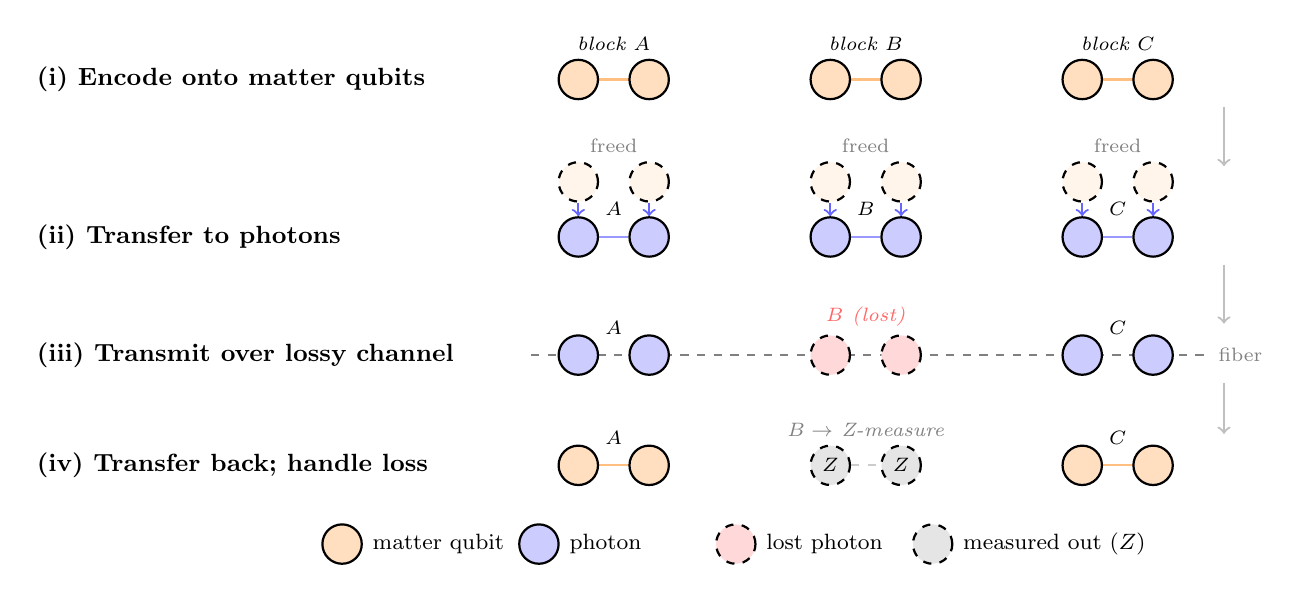
\begin{tikzpicture}[
    qs/.store in    = \qs,    qs    = 0.50cm,
    bsep/.store in  = \bsep,  bsep  = 0.9cm,
    gsep/.store in  = \gsep,  gsep  = 3.2cm,
    rsep/.store in  = \rsep,  rsep  = 1.0cm,
    MQ/.style  = {circle, draw, thick, minimum size=\qs, inner sep=0pt, fill=orange!25},
    PH/.style  = {circle, draw, thick, minimum size=\qs, inner sep=0pt, fill=blue!20},
    LO/.style  = {circle, draw, thick, minimum size=\qs, inner sep=0pt, fill=red!15, dashed},
    MS/.style  = {circle, draw, thick, minimum size=\qs, inner sep=0pt, fill=gray!20, dashed},
    lbl/.style = {font=\small\bfseries, align=left, anchor=west},
    ann/.style = {font=\scriptsize},
    blk/.style = {font=\scriptsize\itshape},
]

% Block qubit x-coords
\def\Ax{0.0}  \def\Bx{0.9}    % block A
\def\Cx{3.2}  \def\Dx{4.1}    % block B
\def\Ex{6.4}  \def\Fx{7.3}    % block C
% Block centres
\def\cA{0.45} \def\cB{3.65} \def\cC{6.85}
% Right margin for step arrows
\def\arrx{8.2}
% Left margin for labels
\def\lblx{-7}
\def\legendOffset{-3}

% Row y-coords
\def\yI{0}
\def\yII{-2}
\def\yIII{-3.5}
\def\yIV{-4.9}
\def\yV{-5.9}

%% ══════════════════════════════════════════════════
%% ROW (i)
%% ══════════════════════════════════════════════════
\node[lbl] at (\lblx, \yI) {(i) Encode onto matter qubits};

\foreach \xa/\xb/\lbl in {\Ax/\Bx/A, \Cx/\Dx/B, \Ex/\Fx/C}{
    \draw[thick, orange!50] (\xa,\yI)--(\xb,\yI);
    \node[MQ] at (\xa, \yI) {};
    \node[MQ] at (\xb, \yI) {};
}
\node[blk, above=7pt] at (\cA,\yI) {block $A$};
\node[blk, above=7pt] at (\cB,\yI) {block $B$};
\node[blk, above=7pt] at (\cC,\yI) {block $C$};

%% ══════════════════════════════════════════════════
%% ROW (ii)
%% ══════════════════════════════════════════════════
\node[lbl] at (\lblx, \yII) {(ii) Transfer to photons};

\def\phshift{0.70}  % photon sits above matter qubit

\foreach \xa/\xb/\bl in {\Ax/\Bx/A, \Cx/\Dx/B, \Ex/\Fx/C}{
    % matter qubits (dashed = freed)
    \node[MQ, fill=orange!8, dashed] (mA) at (\xa, \yII+\phshift) {};
    \node[MQ, fill=orange!8, dashed] (mB) at (\xb, \yII+\phshift) {};
    % photons above
    \node[PH] (pA) at (\xa, \yII) {};
    \node[PH] (pB) at (\xb, \yII) {};
    \draw[thick, blue!40] (pA)--(pB);
    % transfer arrows
    \draw[->, thick, blue!60] (mA.south)--(pA.north)
        node[midway, left, ann]{};
    \draw[->, thick, blue!60] (mB.south)--(pB.north)
        node[midway, right, ann]{};
    \node[ann, gray, above=7pt] at ({(\xa+\xb)/2}, \yII+\phshift) {freed};
    \node[blk, below=4pt] at ({(\xa+\xb)/2}, \yII+\phshift) {$\bl$};
}

%% ══════════════════════════════════════════════════
%% ROW (iii)
%% ══════════════════════════════════════════════════
\node[lbl] at (\lblx, \yIII) {(iii) Transmit over lossy channel};

\draw[dashed, gray, thick] (-0.6, \yIII) -- (8.0, \yIII)
    node[right, ann, gray] {fiber};

% Block A intact
\node[PH] at (\Ax, \yIII) {};
\node[PH] at (\Bx, \yIII) {};
\node[blk, above=4pt] at (\cA, \yIII) {$A$};

% Block B lost
\node[LO] at (\Cx, \yIII) {};
\node[LO] at (\Dx, \yIII) {};
\node[blk, above=7pt, red!60] at (\cB, \yIII) {$B$ (lost)};

% Block C intact
\node[PH] at (\Ex, \yIII) {};
\node[PH] at (\Fx, \yIII) {};
\node[blk, above=4pt] at (\cC, \yIII) {$C$};

%% ══════════════════════════════════════════════════
%% ROW (iv-v)
%% ══════════════════════════════════════════════════
\node[lbl] at (\lblx, \yIV) {(iv) Transfer back; handle loss};

% Block A
\draw[thick, orange!50] (\Ax,\yIV)--(\Bx,\yIV);
\node[MQ] at (\Ax, \yIV) {};
\node[MQ] at (\Bx, \yIV) {};
\node[blk, above=4pt] at (\cA, \yIV) {$A$};

% Block B measured out
\node[MS] (mzA) at (\Cx, \yIV) {};
\node[MS] (mzB) at (\Dx, \yIV) {};
\node[ann] at (mzA) {$Z$};
\node[ann] at (mzB) {$Z$};
\draw[thick, gray!40, dashed] (mzA)--(mzB);
\node[blk, above=7pt, gray] at (\cB, \yIV) {$B\to$ Z-measure};

% Block C
\draw[thick, orange!50] (\Ex,\yIV)--(\Fx,\yIV);
\node[MQ] at (\Ex, \yIV) {};
\node[MQ] at (\Fx, \yIV) {};
\node[blk, above=4pt] at (\cC, \yIV) {$C$};

%% ══════════════════════════════════════════════════
%% ROW (vi)
%% ══════════════════════════════════════════════════
% \node[lbl] at (\lblx, \yV) {(v) Re-encode; forward};

% % Block A' — two matter qubits
% \draw[thick, orange!50] (\Ax,\yV)--(\Bx,\yV);
% \node[MQ] at (\Ax, \yV) {};
% \node[MQ] at (\Bx, \yV) {};
% \node[blk, above=7pt] at (\cA, \yV) {block $A'$};

% % Block B' — two matter qubits
% \draw[thick, orange!50] (\Cx,\yV)--(\Dx,\yV);
% \node[MQ] at (\Cx, \yV) {};
% \node[MQ] at (\Dx, \yV) {};
% \node[blk, above=7pt] at (\cB, \yV) {block $B'$};

% % Block C' — two matter qubits
% \draw[thick, orange!50] (\Ex,\yV)--(\Fx,\yV);
% \node[MQ] at (\Ex, \yV) {};
% \node[MQ] at (\Fx, \yV) {};
% \node[blk, above=7pt] at (\cC, \yV) {block $C'$};

% \node[ann, gray, below=7pt] at (\cB, \yV)
%     {re-encoded to original size $\to$ next hop};

%% ══════════════════════════════════════════════════
%% Step arrows (right margin)
%% ══════════════════════════════════════════════════
\draw[->, thick, gray!50] (\arrx, \yI-0.35)   -- (\arrx, \yII+0.9);
\draw[->, thick, gray!50] (\arrx, \yII-0.35)  -- (\arrx, \yIII+0.4);
\draw[->, thick, gray!50] (\arrx, \yIII-0.35) -- (\arrx, \yIV+0.4);
% \draw[->, thick, gray!50] (\arrx, \yIV-0.35)  -- (\arrx, \yV+0.4);

%% ══════════════════════════════════════════════════
%% Legend
%% ══════════════════════════════════════════════════
\begin{scope}[shift={(\legendOffset, \yV)}] %-1.1
    \node[MQ, label=right:{\footnotesize matter qubit}]     at (0.0, 0) {};
    \node[PH, label=right:{\footnotesize photon}]           at (2.5, 0) {};
    \node[LO, label=right:{\footnotesize lost photon}]      at (5.0, 0) {};
    \node[MS, label=right:{\footnotesize measured out ($Z$)}] at (7.5, 0) {};
\end{scope}

\end{tikzpicture}